% ============================================================
% Mechanistic Validity: Scientific Formalization and Theory of
% Validity for Interpretability Claims
% ============================================================
\pdfoutput=1

% NOTE: This paper is intended for TMLR format.
% If tmlr.sty is available, use:
%   \documentclass[10pt]{article}
%   \usepackage[preprint]{tmlr}
% Otherwise, the following provides compatible formatting.
\documentclass[10pt]{article}

% --- Try TMLR style; fall back to compatible packages ---
\IfFileExists{tmlr.sty}{%
  \usepackage[preprint]{tmlr}%
}{%
  \usepackage[margin=1in]{geometry}%
  \usepackage{times}%
  \usepackage{authblk}%
}

\usepackage[T1]{fontenc}
\usepackage[utf8]{inputenc}
\usepackage{microtype}
\usepackage{amsmath,amssymb}
\usepackage{booktabs}
\usepackage{graphicx}
\graphicspath{{figures/}}
\usepackage{xcolor}
\usepackage{hyperref}
\usepackage{cleveref}
\usepackage{enumitem}
\usepackage{placeins}
\usepackage{float}
\usepackage{multirow}
\usepackage{array}
\usepackage{natbib}

% --- Macros ---
\newcommand{\mechval}{\textsc{MechVal}}
\newcommand{\ie}{i.e.}
\newcommand{\eg}{e.g.}
\newcommand{\cf}{cf.}

% tight tables
\newcommand{\tighttable}{\setlength{\tabcolsep}{4pt}\renewcommand{\arraystretch}{1.05}}

% add space between caption and table rule
\usepackage{caption}
\captionsetup[table]{skip=8pt}

\title{Mechanistic Validity: A Theory of Validity for Interpretability Claims}

\IfFileExists{tmlr.sty}{}{%
  \author[1]{Elliot Tower}
  \affil[1]{Independent Researcher, \texttt{elliot@elliottower.com}}
  \date{}
}

\begin{document}

\maketitle

% ============================================================
\begin{abstract}
A mechanistic explanation of a neural network is not a single experimental result, but a structured claim linking a theoretical construct, a measurement procedure, an intervention, and a scope of interpretation. We introduce Mechanistic Validity (\mechval{}), a formalized epistemology for validating these causal claims, drawing on validation methodology from causal inference, measurement theory, and the philosophy of science. The framework makes interpretability claims explicit, falsifiable, and comparable, formalizing the discovery, validation, and interpretation of causal mechanisms as separate evidential stages. A central problem the framework addresses is that post-hoc mechanistic narratives are unfalsifiable: given any set of ablation results, a plausible story can always be constructed to fit them. \mechval{} organizes 27 operational criteria across five validity types---construct, measurement, internal, external, and interpretive---in dependency order, and assigns each claim to one of five verdict tiers from Proposed to Validated. The criteria make the absence of falsification tests visible in the validity profile. The framework is method-agnostic, applying the same criteria to circuits, SAE features, probing classifiers, steering vectors, transcoders, and crosscoders, and is supported by an open-source implementation with 84 metrics across five evidence families and 14 calibrations. Claims are additionally qualified by one of Marr's \citeyearpar{marr1982vision} three canonical levels of description---computational, algorithmic, and implementational---which we extend with representational as a fourth level and with four implementational sub-types: topographic, connectomic, activation-statistical, and functional. Applying the framework to 13 published circuits, we show that the tier system discriminates among claims---from Proposed (SAE features, probing classifiers) to Triangulated (induction heads, grokking)---with every verdict traceable to specific present or missing evidence. By making the evidential status of a claim explicit and the path to strengthening it concrete, \mechval{} aims to help interpretability mature into a discipline whose claims are both interpretable and scientifically validated.
\end{abstract}

% ============================================================
\section{Introduction}
\label{sec:intro}

Mechanistic interpretability has produced a remarkable catalog of internal mechanisms:
induction heads that implement in-context copying \citep{olsson2022context}, a multi-role
circuit for indirect object identification \citep{wang2023interpretability}, a greater-than
algorithm \citep{hanna2023greater}, and sparse autoencoder features proposed to correspond
to human-interpretable concepts \citep{cunningham2023sparse}. The field has also begun to
build evaluation infrastructure: faithfulness metrics for circuits
\citep{miller2024transformer}, the Mechanistic Interpretability Benchmark for comparing
localization methods across tasks and models \citep{mueller2025mib}, SAEBench for auditing
sparse autoencoder quality \citep{karvonen2025saebench}, and causal scrubbing for testing
mechanistic hypotheses via behavior-preserving resampling \citep{chan2022causal}.

These contributions evaluate important objects---methods, circuits, features, alignments,
benchmark scores. They do not by themselves answer a different question: what has been
established by a mechanistic interpretability \emph{claim}? A claim such as ``this head is
a name mover,'' ``this feature represents deception,'' or ``this subspace implements a
causal variable'' is not just a circuit or a metric value. It links a theoretical
construct to a measurement procedure, a causal intervention, a scope of generalization,
and a natural-language interpretation. Shared metrics are not yet shared validity criteria.

A mechanistic narrative that was retrofitted to match ablation results is currently
indistinguishable from one that has survived refutation attempts. This matters because a
mechanistic explanation has many adjustable parts---which components to include, what roles
to assign, which edges to draw---and a narrative with enough flexibility will always fit
the observations. The \mechval{} framework introduced below provides the criteria needed to
distinguish well-supported claims from plausible-sounding ones, making the gaps in evidence
visible rather than leaving them implicit.

Several recent results sharpen this point. \citet{sutter2025nonlinear} prove that without
structural constraints on alignment maps, causal abstraction becomes vacuous: sufficiently
expressive maps can perfectly align randomly initialized language models to arbitrary
algorithms, achieving 100\% interchange-intervention accuracy on tasks the models cannot
solve. The SAEBench audit reveals that two of six standard SAE evaluation metrics fail
basic diagnostics for reseed stability, ground-truth correlation, and discriminability
\citep{karvonen2025saebench}. And execution-grounded reproducibility checks via
MechEvalAgent \citep{bai2026mecheval} surface claim-evidence coherence issues that
narrative review misses. Each finding bears on a different link in the inference chain:
alignment-map complexity, measurement reliability, and reproducibility, respectively. What
is missing is not any one fix but a principled way to ask, of any claim, which links have
been established and which have not.

We introduce \mechval{}, a formalized epistemology for validating mechanistic
interpretability claims, drawing on validation methodology from causal inference,
measurement theory, and the philosophy of science. The framework makes interpretability
claims explicit, falsifiable, and comparable, formalizing the discovery, validation, and
interpretation of causal mechanisms as separate evidential stages. It defines 27
operational criteria across five validity types---construct, measurement, internal,
external, and interpretive---in dependency order, with five verdict tiers marking
qualitative transitions in evidential status.

\mechval{} is claim-centric and method-agnostic: it evaluates circuits, SAE features,
probing classifiers, steering vectors, transcoders, and crosscoders with the same
criteria. A faithfulness score, an interchange-intervention accuracy, a probe accuracy, or
a causal-scrubbing result can all serve as evidence within the framework; the framework
specifies what kind of evidence each provides, what kind of claim it can support, and what
remains untested. \mechval{} does not replace existing benchmarks or methods. It provides a
common layer above them: claim-level validation built on method-level evaluation.

We describe the framework (\Cref{sec:framework}), its theoretical foundations
(\Cref{sec:foundations}), its application to 13 published circuits
(\Cref{sec:case-studies}), and its implications for the field (\Cref{sec:discussion}).

% ============================================================
\section{Related Work}
\label{sec:related}

Three recent efforts assess different layers of the MI evidence stack, and \mechval{} is designed to complement rather than replace them.

The Mechanistic Interpretability Benchmark (MIB; \citealp{mueller2025mib}) compares circuit-discovery and causal-variable-localization methods on a shared task suite using Circuit Model Distance and Interchange Intervention Accuracy. MIB is method-vs-method: given a task, which discovery algorithm produces the best circuit? \mechval{} is method-agnostic and claim-centric: given a claim about how a model works, what evidence would be needed to sustain it? The two are stacked rather than competing---MIB scores a method's output on a single dimension, while \mechval{} assesses how that output is interpreted, generalized, and reported.

SAEBench \citep{karvonen2025saebench} evaluates sparse autoencoders along six metric families and audits the metrics themselves. Two of six metrics (TPP, SCR) fail diagnostic tests for reseed stability, ground-truth correlation, and discriminability, motivating the explicit measurement-validity dimension in our framework. \mechval{} treats SAEBench's audit as evidence \emph{about} the M-dimension criteria (M1 reliability, M5 sensitivity, M6 invariance) rather than as a competing benchmark.

MechEvalAgent \citep{bai2026mecheval} performs execution-grounded reproducibility checks on published MI papers, finding that 93\% fail to reproduce when their code is run and that 80\% fail claim-evidence coherence checks. Where MechEvalAgent asks ``does this code run and match its prose?,'' \mechval{} asks ``does this evidence pattern support this kind of claim?''

Finally, the LLM-as-judge paradigm \citep{zheng2023judging} has been applied to open-ended evaluation of MI research. However, unstructured LLM evaluation lacks the operational criteria needed to distinguish genuine validity from surface plausibility---the same limitation that affects human narrative review, as demonstrated by MechEvalAgent's finding that narrative review misses issues that execution-grounded checks catch.

A companion paper automates \mechval{} via structured LLM extraction against the 27 criteria, and describes protocols (curated experiment designs that bundle metrics around specific validity questions) and synthesis algorithms (aggregation across evidence families to produce quantitative scores). Automation and scoring are treated separately because the framework's correctness is independent of whether verdicts are assigned by hand or by machine.

\begin{figure}[H]
\centering
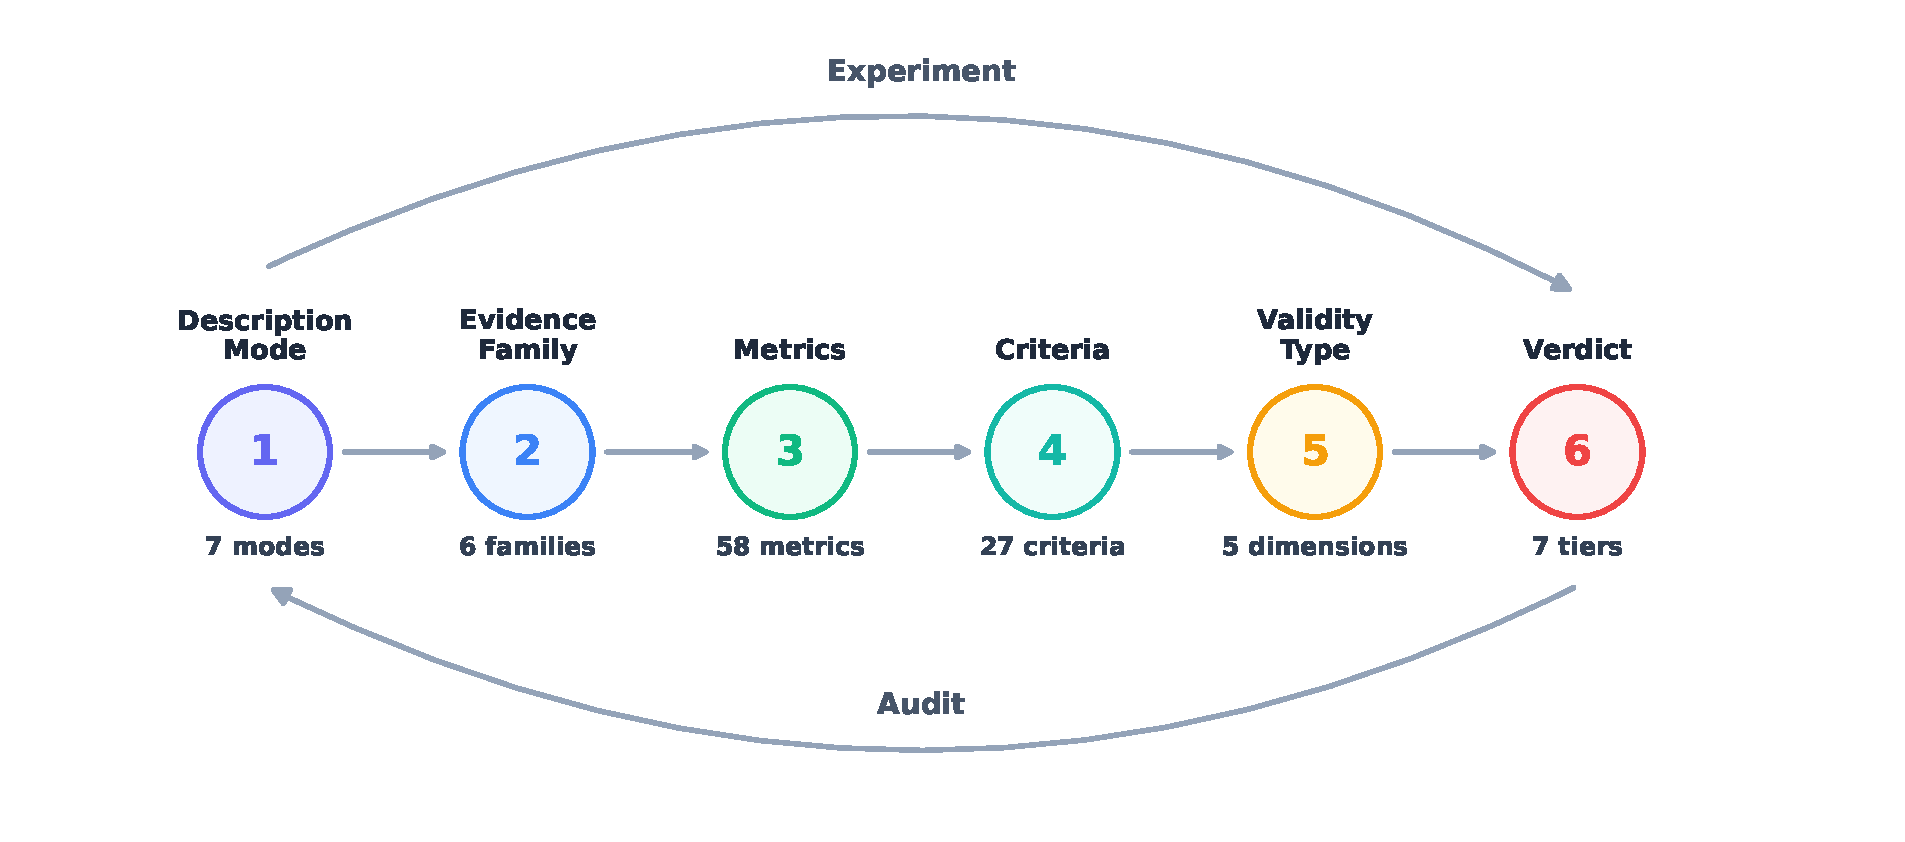
\includegraphics[width=\linewidth]{pipeline-final.pdf}
\caption{The \mechval{} framework hierarchy. Six layers from description mode through verdict. \textbf{Experiment} (left-to-right): from raw measurements, build upward through criteria and validity types to a verdict. \textbf{Audit} (right-to-left): given a claimed verdict, trace backward to identify which lower-layer criteria are unmet.}
\label{fig:pipeline}
\end{figure}

% ============================================================
\section{From Claim to Verdict}
\label{sec:overview}

Consider a concrete claim: ``The IOI circuit uses three name-mover heads (9.9, 9.6, 10.0) to copy the indirect object to the output position.'' This claim appears in a widely-cited paper, is supported by ablation experiments, and has a clear mechanistic narrative. What has this claim established, and what remains untested?

The framework evaluates such a claim through six layers (\Cref{fig:pipeline}):

\begin{enumerate}[nosep]
\item \textbf{Description mode.} At what level is the claim made? The IOI claim operates at the implementational-functional level: it names specific heads and says what each one does. A weaker claim (``GPT-2 solves IOI'') would be computational; a stronger one (``head 9.9 implements copying via its OV circuit'') would require additional structural evidence.

\item \textbf{Evidence family.} What kinds of evidence are available? The original IOI paper provides primarily causal evidence (ablation) and some behavioral evidence (faithfulness). Structural evidence (weight-space analysis of the OV circuits) and cross-model evidence (does the same circuit appear in GPT-2 Medium?) would strengthen the claim by adding independent failure modes.

\item \textbf{Metrics.} Which concrete tests were run? Activation patching, role ablation, faithfulness scores. Each metric belongs to an evidence family and produces a measurement that feeds into criteria evaluation.

\item \textbf{Criteria.} Does the evidence meet the bar? The IOI circuit passes necessity (I1: ablation degrades performance) and sufficiency (I2: the circuit alone recovers 87\% of logit difference). But specificity (I3: does the circuit affect \emph{only} IOI?) is untested, and the 87\% faithfulness number is method-conditional---it drops below 50\% under non-mean-ablation methods \citep{miller2024transformer}, partially failing intervention reach (E1).

\item \textbf{Validity type.} Which validity dimensions are satisfied? Construct validity (the claim is well-defined), partial internal validity (necessity and sufficiency shown but specificity untested), partial external validity (limited prompt generalization, no cross-model replication). Measurement validity is unaddressed---no calibration of the ablation metrics themselves.

\item \textbf{Verdict.} What tier does the claim reach? Mechanistically Supported---necessity and sufficiency are established with at least one method, but the evidence comes primarily from one methodological family (ablation-based), key criteria remain untested (I3, I4, E4), and the faithfulness result is method-conditional. The verdict is not a judgment on the paper's quality; it is a precise characterization of what has been established and what has not.
\end{enumerate}

The 27 criteria also formalize common failure modes observed in published MI research. \Cref{tab:failures} maps twelve such failures to the criteria that detect them.

\begingroup
\small
\begin{table}[H]
\centering
\caption{Taxonomy of common failure modes in MI research and the criteria that detect them.}
\label{tab:failures}
\renewcommand{\arraystretch}{1.15}
\begin{tabular}{@{}l>{\raggedright\arraybackslash}p{3.2cm}>{\raggedright\arraybackslash}p{2.8cm}>{\raggedright\arraybackslash}p{4.0cm}@{}}
\toprule
\textbf{Failure mode} & \textbf{What happens} & \textbf{Criterion} & \textbf{Example} \\
\midrule
Cherry-picking metrics & Run multiple ablation methods, report only the best number & E1 Intervention\newline reach & IOI: 87\% mean ablation reported; resample ablation (40\%) omitted \\
\midrule
No baseline control & Report high score without testing a random or untrained model & M2 Baseline\newline separation & Nonlinear alignment maps achieve 95\% IIA on random models \citep{sutter2025nonlinear} \\
\midrule
No negative controls & Only test predictions that should pass; never test what the mechanism should \emph{not} affect & I3 Specificity\newline C1 Falsifiability & IOI: no test of whether the circuit also degrades SVA or factual recall \\
\midrule
Construct incoherence & Target construct is not separable from a neighboring one & C4 Discriminant\newline validity & Gender bias circuits: bias and knowledge share the same heads \\
\midrule
Off-target effects & Ablation works for the target task; other tasks never checked & I3 Specificity & Knowledge neurons: editing one fact corrupts related facts (ripple effects) \\
\midrule
Circuit redefinition & Drop heads that hurt faithfulness, call it ``refined'' & C1 Falsifiability & Adjusting circuit membership to maximize the target metric \\
\midrule
Post-hoc role labeling & Name heads after observed behavior; the label cannot fail & C1 Falsifiability & ``Name mover'' assigned after seeing logit attribution \\
\midrule
No double dissociation & Show necessity but never test the converse & I4 Double\newline dissociation & IOI circuit ablated $\to$ IOI breaks; SVA circuit $\to$ IOI intact never tested \\
\midrule
Interpretive inflation & Label implies intent or algorithm beyond what evidence shows & V4 Anthropo-\newline morphism check & ``World model'' for Othello (evidence supports ``linearly decodable'') \\
\midrule
Scope creep & Validate on one prompt format, claim generality & V5 Scope decl.\newline E2 Prompt gen. & ``The IOI circuit'' tested only on two-name templates \\
\midrule
Flexible scope & Narrow the claim after seeing results so it cannot fail & V5 Scope\newline declaration & Restricting scope post-hoc to the subset of prompts that work \\
\midrule
Ignoring alternatives & Circuit works, but so does a different set of heads & I4 Double dissoc.\newline C3 Convergent val. & Meloux et al.\ find alternative IOI circuits with comparable faithfulness \\
\bottomrule
\end{tabular}
\end{table}
\endgroup


% ============================================================
\section{The Framework}
\label{sec:framework}

The \mechval{} framework has six layers, presented here in pipeline order (\Cref{fig:pipeline}): description modes (\Cref{sec:description-modes}), evidence families (\Cref{sec:evidence-families}), metrics (\Cref{sec:metrics}), criteria (\Cref{sec:criteria}), validity types (\Cref{sec:validity-types}), and verdict tiers (\Cref{sec:verdict-tiers}).

\subsection{Description Modes}
\label{sec:description-modes}

MI claims operate at different levels of description, following Marr's hierarchy but adapted for transformer circuits. The framework defines seven description modes (\Cref{tab:modes}) forming a partial order by evidential commitment. Higher modes require all evidence from lower modes plus bridging evidence that connects levels. A claim at the algorithmic level (``the model runs a detect-inhibit-copy algorithm'') requires both the topographic evidence (which heads are involved) and the additional evidence that the heads implement the claimed algorithm. Mode tags are applied to verdicts, not to individual metrics---a single experiment can provide evidence for multiple modes simultaneously.

\begin{table}[H]
\centering
\small
\caption{The seven description modes.}
\label{tab:modes}
\renewcommand{\arraystretch}{1.2}
\begin{tabular}{@{}rl>{\raggedright\arraybackslash}p{4.8cm}>{\raggedright\arraybackslash}p{5.2cm}@{}}
\toprule
& \textbf{Mode} & \textbf{What it asks} & \textbf{Example} \\
\midrule
1 & Computational & What function does the system compute, and why? & ``GPT-2 predicts the indirect object'' \\
\midrule
2 & Algorithmic & What procedure does it execute? & ``A detect-inhibit-copy algorithm'' \\
\midrule
3 & Representational & What information is encoded, and in what geometry? & ``The IO name is linearly encoded at layer 8'' \\
\midrule
4 & Impl.-Functional & What transformation does each component perform? & ``Head 9.9 copies names to the output'' \\
\midrule
5 & Impl.-Connectomic & How are components wired? & ``S-inhibition feeds name movers via residual stream'' \\
\midrule
6 & Impl.-Topographic & Which components are involved? & ``Heads 9.9, 9.6, 10.0'' \\
\midrule
7 & Impl.-Statistical & What do activations look like? & ``Head 9.9 attends strongly to IO position'' \\
\bottomrule
\end{tabular}
\end{table}

\subsection{Evidence Families}
\label{sec:evidence-families}

An evidence family classifies a metric's output by the kind of signal it produces, independent of the specific tool used to generate it (\Cref{tab:families}). The classification matters because convergent validity---two independent lines of evidence agreeing---is the strongest form of support for a mechanistic claim. But not all agreement is equally informative: two causal metrics agreeing shares failure modes, while a causal ablation and a structural weight-space analysis agreeing is substantially stronger, because a confound that fools one family cannot fool the other.

\begin{table}[H]
\centering
\small
\caption{The six evidence families.}
\label{tab:families}
\renewcommand{\arraystretch}{1.2}
\begin{tabular}{@{}ll>{\raggedright\arraybackslash}p{4.5cm}>{\raggedright\arraybackslash}p{5cm}@{}}
\toprule
& \textbf{Family} & \textbf{What it measures} & \textbf{Examples} \\
\midrule
A & Causal & Effects of interventions on computation & Activation patching, DAS-IIA, CATE, mediation \\
\midrule
B & Structural & Weight-space properties (no forward pass) & SVD, effective rank, OV/QK composition \\
\midrule
C & Information & Information flow and dependencies & Mutual information, PID, OCSE, transfer entropy \\
\midrule
D & Behavioral & Input-output behavior under manipulation & Faithfulness, logit diff, KL divergence, dose-response \\
\midrule
E & Representational & Geometry of internal representations & CKA, RSA, linear probes, attention entropy \\
\midrule
F & Measurement & Trustworthiness of other metrics & Bootstrap stability, seed variance, convergent validity \\
\bottomrule
\end{tabular}
\end{table}

The framework tracks evidence family coverage explicitly: a claim supported by three families is stronger than one supported by three metrics from the same family.

\subsection{Metrics}
\label{sec:metrics}

Metrics are runnable tests that produce measurements about a neural network. They form the empirical base of the framework: evidence families organize them, criteria evaluate them, and verdicts aggregate them. The current implementation includes 84 metrics across families A--E and 14 calibrations in family F. \Cref{tab:causal_metrics} illustrates the causal family; the full inventory for all six families is in \Cref{app:metrics}.

\begin{table}[H]
\centering
\small
\caption{Causal metrics (family A): effects of interventions on model computation.}
\label{tab:causal_metrics}
\renewcommand{\arraystretch}{1.15}
\begin{tabular}{@{}l>{\raggedright\arraybackslash}p{9.5cm}@{}}
\toprule
\textbf{Metric} & \textbf{Description} \\
\midrule
A01 SCM / Pearl & Structural causal models and do-calculus as the formal language for circuit claims \\
\midrule
A02 Counterfactual DAS & Distributed Alignment Search and IIA for testing causal abstraction hypotheses \\
\midrule
A03 Rubin CATE & Conditional average treatment effects across input subpopulations \\
\midrule
A04 Woodward & Interventionist theory of causation applied to circuit ablation \\
\midrule
A05 MDC / Glennan & New mechanical philosophy: components organized to produce phenomena \\
\midrule
A06 Mediation & Natural direct and indirect effects decomposition for circuit paths \\
\midrule
A07 Granger / TE & Observational causal discovery via conditional MI and temporal precedence \\
\midrule
A08 PID & Decomposing MI into redundant, unique, and synergistic contributions \\
\midrule
A09 MDL / SLT & Minimum description length and singular learning theory for circuit complexity \\
\midrule
A10 Regularity / INUS & INUS conditions: insufficient but necessary parts of sufficient sets \\
\midrule
A11 Actual Cause & Halpern-Pearl actual causation on specific inputs, not just potential causes \\
\midrule
A12 Transportability & Formal conditions for circuit generalization across models and distributions \\
\midrule
A13 Causal Discovery & NOTEARS / PC algorithms for learning DAGs over circuit components \\
\bottomrule
\end{tabular}
\end{table}

\subsection{Criteria}
\label{sec:criteria}

Each validity type is operationalized through specific criteria, totaling 27 across the five validity types. \Cref{tab:criteria} lists all criteria. Each criterion has a concrete test: a claim either passes, partially passes, or fails each criterion, producing a structured validity profile rather than a single score.

\begingroup
\hyphenpenalty=10000
\exhyphenpenalty=10000
\begin{table}[H]
\centering
\small
\caption{The 27 criteria across five validity types.}
\label{tab:criteria}
\renewcommand{\arraystretch}{1.15}
\begin{tabular}{@{}llp{8.5cm}@{}}
\toprule
\textbf{ID} & \textbf{Criterion} & \textbf{Description} \\
\midrule
C1 & Falsifiability & Can the claim be refuted? \\
C2 & Structural plausibility & Is the mechanism physically possible in the architecture? \\
C3 & Convergent validity & Do multiple independent methods agree? \\
C4 & Discriminant validity & Does the measure distinguish this from neighboring constructs? \\
C5 & Nomological validity & Does the claim fit into a broader theory? \\
\midrule
M1 & Reliability & Do repeated measurements give the same answer? \\
M2 & Baseline separation & Is the score distinguishable from random/untrained baselines? \\
M3 & Stability & Is the classification robust to perturbation? \\
M4 & Calibration & Are the numbers meaningful? \\
M5 & Sensitivity & Can the instrument detect known-true effects? \\
M6 & Invariance & Does the metric behave consistently across conditions? \\
\midrule
I1 & Necessity & Is the circuit required for the behavior? \\
I2 & Sufficiency & Is the circuit enough to produce the behavior? \\
I3 & Specificity & Does the circuit do this task and not everything? \\
I4 & Double dissociation & Can this circuit be separated from other circuits? \\
I5 & Confound control & Are alternative explanations ruled out? \\
\midrule
E1 & Intervention reach & Do different intervention methods agree? \\
E2 & Prompt generalization & Does it work on diverse prompts? \\
E3 & Cross-task generalization & Does the mechanism transfer to related tasks? \\
E4 & Cross-model generalization & Does the mechanism appear in other models? \\
E5 & Graded response & Does partial ablation produce partial effects? \\
E6 & Novel prediction & Does the mechanism predict new, untested behaviors? \\
\midrule
V1 & Level declaration & At what description mode is the claim made? \\
V2 & Level-evidence match & Does the evidence support claims at that level? \\
V3 & Alternative level & Could the evidence be explained at a different level? \\
V4 & Anthropomorphism check & Is the interpretation projecting human concepts? \\
V5 & Scope declaration & What does the claim explicitly not cover? \\
\bottomrule
\end{tabular}
\end{table}
\endgroup

\subsection{Validity Types}
\label{sec:validity-types}

The five validity types form a dependency chain: later types cannot be established without first satisfying earlier ones.

\begin{equation}
\text{Construct} \rightarrow \text{Measurement} \rightarrow \text{Internal} \rightarrow \text{External} \rightarrow \text{Interpretive}
\label{eq:dependency}
\end{equation}

Each type addresses a distinct question about the claim:

\paragraph{Construct validity.} Is the thing being measured well-defined? Before any measurement is taken, the construct must be specified precisely enough that the claim is falsifiable, structurally plausible, and distinguishable from neighboring constructs. A ``deception feature'' that cannot be distinguished from an ``uncertainty feature'' fails construct validity regardless of how carefully it is measured. This draws on philosophy of science (Popper's falsifiability, Hempel's operationalism) and psychometrics (construct validity, convergent and discriminant validity).

\paragraph{Measurement validity.} Are the instruments trustworthy? Once the construct is defined, the measurement tools used to detect it must be reliable (stable across repetitions), calibrated (separable from random baselines), and invariant (consistent across conditions). A metric that gives different answers when run with different random seeds is not evidence. This draws on psychometrics (test-retest reliability, measurement invariance) and pharmacology (assay validation).

\paragraph{Internal validity.} Does the evidence support the causal claim? Given a well-defined construct and trustworthy instruments, the evidence must establish that the identified component is causally involved in the behavior---not merely correlated with it. This requires demonstrating necessity (the component is required), sufficiency (the component is enough), and specificity (the component does this task and not everything). This draws on neuroscience (lesion studies, optogenetics, double dissociation) and causal inference \citep{pearl2009causality}.

\paragraph{External validity.} Does the mechanism generalize? Causal evidence on one prompt set, with one ablation method, in one model, establishes internal validity at best. External validity requires that the mechanism generalizes across prompts, ablation methods, related tasks, and ideally across models. This draws on pharmacology (Phase~III generalization, dose-response) and causal inference (transportability; \citealp{pearl2011transportability}).

\paragraph{Interpretive validity.} Is the interpretation of the mechanism correct? Finally, the natural-language description of the mechanism must be justified by the evidence. A head called a ``name mover'' based on direct logit attribution carries theoretical implications beyond what the evidence strictly supports. Interpretive validity requires declaring the description level, matching evidence to that level, and checking for anthropomorphic inflation. This is specific to MI but draws on Marr's levels of analysis \citep{marr1982vision}.

\subsection{Verdict Tiers}
\label{sec:verdict-tiers}

Claims are assigned to one of five verdict tiers representing qualitative transitions in evidential status. Two additional labels handle special cases. The tiers form a strict hierarchy: each requires all evidence from the tier below plus additional evidence.

\begin{table}[t]
\centering
\tighttable
\caption{Verdict tiers with requirements. Each tier subsumes the requirements of all lower tiers.}
\label{tab:verdicts}
\small
\begin{tabular}{@{}lp{4.5cm}p{5.5cm}@{}}
\toprule
\textbf{Tier} & \textbf{Meaning} & \textbf{Requirements beyond previous tier} \\
\midrule
Proposed & Structural or representational evidence only & Construct validity criteria met (C1--C5) \\
Causally Suggestive & Necessity shown, sufficiency not established & Internal validity I1 (necessity via ablation) \\
Mechanistically Supported & Necessity + sufficiency with consistent methods & I1 + I2 (sufficiency), intervention reach (E1), at least 2 ablation variants \\
Triangulated & Multiple converging lines of independent evidence & Full internal + external + construct criteria from $\geq 3$ evidence families \\
Validated & All five validity types addressed & Measurement + interpretive validity with explicit baselines \\
\midrule
Underdetermined & Evidence consistent with multiple mechanisms & Cannot resolve between rival specifications \\
Disconfirmed & Fails decisively on a key criterion & Negative result \\
\bottomrule
\end{tabular}
\end{table}

Every tier carries a specific epistemic meaning: a claim at \emph{Proposed} is not a failed claim but one whose evidential status---and the path to strengthening it---is precisely characterized. The verdict tells researchers exactly what additional evidence would advance the claim: a Proposed claim needs causal intervention (I1) to reach Causally Suggestive; a Causally Suggestive claim needs sufficiency evidence (I2) and method consistency (E1) to reach Mechanistically Supported.

% ============================================================
\section{Theoretical Foundations}
\label{sec:foundations}

Each component of the framework is grounded in an established validation tradition. The 27 criteria, the dependency chain among validity types, and the verdict tier system are not novel inventions---they are adaptations of principles that have been tested and refined across decades of methodological work in five fields.

\subsection{Philosophy of Science}
\label{sec:phil-sci}

The construct validity criteria (C1--C5) draw on Popper's falsifiability criterion, Mayo's severe testing \citep{mayo2018statistical}, and Glennan's new mechanical philosophy \citep{glennan2017new}. A key distinction is between \emph{confirmation} and \emph{corroboration}: a circuit discovered by activation patching and evaluated by activation patching has only been shown to pass the test it was built to pass. Corroboration requires a genuinely risky test the circuit was not optimized for---a behavioral prediction on held-out prompts, a weight-space analysis, a different causal method. The verdict tier system reflects this hierarchy: single-method evidence (Causally Suggestive) is qualitatively weaker than convergent evidence from independent methods (Triangulated).

C5 (nomological validity) requires that the claim fit into a broader theoretical network, following Cronbach and Meehl's nomological network concept. The Duhem-Quine underdetermination problem is directly relevant: multiple circuits with low overlap can each individually pass faithfulness tests, and reporting this explicitly is a stronger finding than suppressing it.

\begin{table}[H]
\centering\small
\caption{Philosophy of science foundations.}
\renewcommand{\arraystretch}{1.12}
\begin{tabular}{@{}l>{\raggedright\arraybackslash}p{2cm}l>{\raggedright\arraybackslash}p{4.5cm}@{}}
\toprule
\textbf{Concept} & \textbf{Source} & \textbf{Criterion} & \textbf{MI analog} \\
\midrule
Falsifiability & Popper 1959 & C1 & What evidence would refute ``this is a name mover''? \\
\midrule
Nomological network & Cronbach \& Meehl 1955 & C5 & Does the claim connect to in-context learning theory? \\
\midrule
MTMM matrix & Campbell \& Fiske 1959 & C3, C4 & Convergent: probing + patching agree. Discriminant: feature $\neq$ neighboring feature \\
\midrule
Underdetermination & Duhem 1906 & I4 & Multiple circuits explain the same behavior \\
\midrule
Severe testing & Mayo 2018 & C1 & A test that could easily have failed but did not \\
\bottomrule
\end{tabular}
\end{table}

\subsection{Neuroscience}
\label{sec:neuro}

The internal validity criteria (I1--I5) are adapted from neuroscience's toolkit for establishing that a neural circuit implements a computation. I1 (necessity) corresponds to lesion studies; I2 (sufficiency) to stimulation; I4 (double dissociation) is the gold standard for functional specificity \citep{woodward2003making}. The critical distinction between necessity and sufficiency---well-established in neuroscience but often elided in MI---is central to the framework and marks a qualitative transition between verdict tiers.

A less appreciated requirement is Craver's \emph{mutual manipulability}: constitutive relevance requires not only that intervening on the component changes the behavior, but that intervening on the behavior changes the component's activity. The second direction---does fine-tuning away IOI capability cause name-mover heads to lose their OV copying structure?---is almost never tested in MI, yet it is what ``implementation'' actually requires. Additionally, the \emph{parcellation problem} is directly relevant: neuroscience learned that the right unit of analysis is defined by convergence across independent modalities, not by any single method. When EAP, weight classification, and ablation disagree on component membership, the ``circuit'' is probably method-dependent.

\begin{table}[H]
\centering\small
\caption{Neuroscience foundations.}
\renewcommand{\arraystretch}{1.12}
\begin{tabular}{@{}l>{\raggedright\arraybackslash}p{2cm}l>{\raggedright\arraybackslash}p{4.5cm}@{}}
\toprule
\textbf{Concept} & \textbf{Source} & \textbf{Criterion} & \textbf{MI analog} \\
\midrule
Lesion studies & Shallice 1988 & I1 & Ablation degrades behavior \\
\midrule
Double dissociation & Shallice 1988 & I4 & Circuit A breaks task X not Y; circuit B breaks Y not X \\
\midrule
Mutual manipulability & Craver 2007 & I3 & Fine-tuning away the task changes the component \\
\midrule
Multimodal parcellation & Glasser et al.\ 2016 & C3 & Circuit boundaries should converge across methods \\
\midrule
Neural manifolds & Gallego et al.\ 2017 & V2 & Representation geometry constrains algorithmic claims \\
\bottomrule
\end{tabular}
\end{table}

\subsection{Psychometrics}
\label{sec:psychometrics}

The measurement validity criteria (M1--M6) draw on psychometric test construction. Classical test theory decomposes an observed score into true score plus error ($X = T + E$); M1 (reliability) is the proportion of true-score variance. Generalizability theory extends this by decomposing error into distinct sources---prompt variation, random seed, checkpoint selection---each of which can be quantified and reduced independently.

A crucial insight is that a reliable metric pointed at the wrong target produces confident wrong answers. \citet{sutter2025nonlinear} demonstrated this formally: unconstrained nonlinear IIA achieves near-perfect scores on randomly initialized models. The metric is working correctly; it is measuring the alignment map's flexibility, not the model's representational geometry. The framework addresses this through M2 (baseline separation): not ``IIA = 0.48'' but ``$\Delta_{\text{random}} = 0.10$, $\Delta_{\text{untrained}} = 0.15$.'' A modest absolute number with a large delta is a genuine finding; a large absolute number with a tiny delta is not.

\begin{table}[H]
\centering\small
\caption{Psychometrics foundations.}
\renewcommand{\arraystretch}{1.12}
\begin{tabular}{@{}l>{\raggedright\arraybackslash}p{2.2cm}l>{\raggedright\arraybackslash}p{4.5cm}@{}}
\toprule
\textbf{Concept} & \textbf{Source} & \textbf{Criterion} & \textbf{MI analog} \\
\midrule
Classical test theory & Lord \& Novick 1968 & M1 & Same metric, same model $\to$ same answer \\
\midrule
Generalizability theory & Cronbach et al.\ 1972 & M6 & Decompose variance into prompt/seed/checkpoint \\
\midrule
Signal detection ($d'$) & Green \& Swets 1966 & M2 & Is the score distinguishable from random? \\
\midrule
MTMM matrix & Campbell \& Fiske 1959 & C3, C4 & Convergent + discriminant validity \\
\midrule
Selectivity & Hewitt \& Liang 2019 & I3 & Probe accuracy minus control accuracy \\
\bottomrule
\end{tabular}
\end{table}

\subsection{Pharmacology}
\label{sec:pharma}

The external validity criteria draw on pharmacology's dose-response methodology. A causally relevant component should produce graded effects: partial ablation should produce partial behavioral change, and the relationship should be monotonic or at least systematic (E5). The framework treats dose-response as a minimum bar for causal claims about magnitude---a requirement absent from most MI evaluations, which typically report binary ablation (all-or-nothing).

The \emph{affinity vs.\ efficacy} distinction maps with surprising precision to MI. Activation patching measures affinity: is this component engaged during the task? Ablation measures efficacy: does removing it change the output? But even ablation conflates efficacy with the system's compensatory capacity---a load-bearing head can show small ablation effects if backup mechanisms compensate. The observed effect magnitude is a joint property of the component's role and the network's reserve, and a single ablation cannot separate them. The practical implication is the \emph{therapeutic window}: sweeping ablation strength from 0 to 1 reveals whether there is a range where on-task effects grow before off-target degradation begins. A circuit with no therapeutic window cannot be cleanly separated from the network's general processing.

\begin{table}[H]
\centering\small
\caption{Pharmacology foundations.}
\renewcommand{\arraystretch}{1.12}
\begin{tabular}{@{}l>{\raggedright\arraybackslash}p{2.2cm}l>{\raggedright\arraybackslash}p{4.5cm}@{}}
\toprule
\textbf{Concept} & \textbf{Source} & \textbf{Criterion} & \textbf{MI analog} \\
\midrule
Dose-response curve & Hill 1910 & E5 & Partial ablation $\to$ partial effect \\
\midrule
Affinity vs efficacy & Stephenson 1956 & I1 vs I2 & Participation $\neq$ causation \\
\midrule
System reserve & Black \& Leff 1983 & I2 & Backup circuits compensate after ablation \\
\midrule
Functional selectivity & Kenakin 2004 & E1 & Ablation method determines the finding \\
\midrule
Phase I/II/III trials & --- & Verdict tiers & Calibrate $\to$ establish causality $\to$ generalize \\
\bottomrule
\end{tabular}
\end{table}

\subsection{Causal Inference}
\label{sec:causal}

The internal validity criteria draw on causal inference methodology \citep{pearl2009causality, spirtes2000causation}. The necessity/sufficiency distinction maps to Woodward's interventionist causation \citep{woodward2003making}: necessity (I1) corresponds to ``would the behavior persist if the component were absent?'' and sufficiency (I2) to ``would the component alone produce the behavior?'' Pearl and Bareinboim's transportability theory \citep{pearl2011transportability} provides the formal conditions under which causal findings transfer across settings, grounding E4 (cross-model generalization). Rubin's potential outcomes framework grounds E5 (graded response) by formalizing heterogeneous treatment effects across input subpopulations---not all prompts may respond to ablation equally.

\begin{table}[H]
\centering\small
\caption{Causal inference foundations.}
\renewcommand{\arraystretch}{1.12}
\begin{tabular}{@{}l>{\raggedright\arraybackslash}p{2.5cm}l>{\raggedright\arraybackslash}p{4.2cm}@{}}
\toprule
\textbf{Concept} & \textbf{Source} & \textbf{Criterion} & \textbf{MI analog} \\
\midrule
do-calculus / SCM & Pearl 2009 & I1, I2 & Formal language for ablation claims \\
\midrule
Interventionism & Woodward 2003 & I1 & ``Would behavior persist if component absent?'' \\
\midrule
Transportability & Pearl \& Bareinboim 2011 & E4 & Conditions for circuit generalization across models \\
\midrule
Causal discovery & Spirtes et al.\ 2000 & --- & Learning circuit structure from data \\
\midrule
Potential outcomes & Rubin 1974 & E5 & Heterogeneous effects across input subpopulations \\
\bottomrule
\end{tabular}
\end{table}

% ============================================================
% ============================================================
\section{Case Studies}
\label{sec:case-studies}

We apply the framework to 13 published MI results, evaluating each through all five validity lenses. The case studies are not intended to rank papers---they demonstrate what the framework looks like in practice and show that the tier system discriminates between well-validated and poorly-validated claims. Quantitative per-paper scoring---including the Claim Validity Score, tier-agreement confusion matrix, and per-criterion heatmaps---is the subject of a companion paper; here we keep the analysis qualitative and trace each verdict to specific missing or present evidence.

\subsection{Verdict Assignments}

\Cref{tab:case-studies} presents the verdict assignments. The key finding is that the tier system produces meaningful discrimination: the 13 claims span the full range from Proposed to Triangulated, with verdict differences traceable to specific missing evidence rather than arbitrary scoring.

\begin{table}[H]
\centering
\small
\caption{Verdict assignments for 13 published circuits, sorted by evidential status. Verdicts are based on published evidence as of evaluation date.}
\label{tab:case-studies}
\renewcommand{\arraystretch}{1.2}
\begin{tabular}{@{}l>{\raggedright\arraybackslash}p{3cm}>{\raggedright\arraybackslash}p{7cm}@{}}
\toprule
\textbf{Verdict} & \textbf{Circuit} & \textbf{Key evidence gap} \\
\midrule
Triangulated & Induction Heads & Simple mechanism, broad replication, thick nomological network \\
\midrule
Mechanistically Supported & Greater-Than & Strong structural plausibility; limited prompt generalization \\
\midrule
Mechanistically Supported & Copy Suppression & Unusually clean specificity; sufficiency partially established \\
\midrule
Mechanistically Supported & IOI Circuit & Method-conditional faithfulness (87\% mean ablation, $<$50\% other methods); specificity untested \\
\midrule
Mechanistically Supported & Superposition & Toy-model-only evidence; criteria semi-confirmed rather than confirmed \\
\midrule
Causally Suggestive & Successor Heads & Cross-domain generalization as convergent evidence; ablation method-conditional \\
\midrule
Causally Suggestive & Othello World Model & ``World model'' label exceeds evidence (``linearly decodable''); interpretive inflation \\
\midrule
Causally Suggestive & Docstring Circuit & Label ambiguity: ``variable binding'' vs.\ simpler ``positional copying'' \\
\midrule
Causally Suggestive & Knowledge Neurons & Strong intervention but weak specificity; editing corrupts related facts \\
\midrule
Causally Suggestive & SAE Features & Thin nomological network; features may be dictionary properties, not model properties \\
\midrule
Proposed & Probing Classifiers & Decodability without intervention = no internal validity \\
\midrule
Proposed & Gender Bias Circuits & Construct incoherence: bias and knowledge share circuits \\
\bottomrule
\end{tabular}
\end{table}


\subsection{Illustrative Examples}

We describe three case studies in detail to illustrate how the framework produces its verdicts.

\paragraph{Induction Heads (Triangulated).} \citet{olsson2022context} identify a two-head composition mechanism for in-context copying: previous-token heads attend to the token before a repeated sequence, and induction heads use this signal to predict the next token. The claim reaches Triangulated because it satisfies criteria across multiple independent evidence families. The mechanism has been replicated across model scales and architectures (E4), confirmed through both activation-level and weight-level analysis (C3 convergent validity from different families), and produces clean dose-response effects (E5). The nomological network is thick: the mechanism connects to in-context learning theory, training dynamics, and cross-model structural predictions. The relative simplicity of the mechanism (two functional roles, clear compositional structure) makes each criterion easier to satisfy.

\paragraph{IOI Circuit (Mechanistically Supported).} \citet{wang2023interpretability} identify 26 attention heads forming a six-role circuit for indirect object identification. The circuit demonstrates strong necessity (I1) and sufficiency (I2): running the model with everything outside the circuit mean-ablated recovers 87\% of the full model's logit difference. However, \citet{miller2024transformer} show that this 87\% figure is specific to mean ablation; under other ablation methods, faithfulness drops below 50\%. This method-conditional result partially satisfies E1 (intervention reach) but reveals that the causal claim is weaker than the headline number suggests. Specificity (I3) is untested: the authors do not report whether ablating the IOI circuit degrades unrelated tasks. A formal double-dissociation has not been conducted. The circuit reaches Mechanistically Supported rather than Triangulated because the evidence comes primarily from one methodological family (ablation-based) and key criteria (I3, I4, I5, E4) remain unaddressed.

\paragraph{Probing Classifiers (Proposed).} Linear probing \citep{belinkov2022probing} trains a classifier on activations to test whether a concept is linearly decodable. The core limitation is fundamental: \emph{a measurement without an intervention is a measurement without internal validity}. Probe success establishes that information is decodable from the activation space, but not that the model uses that information during inference. High probe accuracy is consistent with genuine encoding, incidental linear separability in high-dimensional space, and confound encoding (a correlated feature rather than the target). Without causal follow-up (DAS, intervention along the probe direction), the claim cannot advance beyond Proposed. Probing \emph{with} causal follow-up can reach Causally Suggestive; with additional control tasks and cross-method convergence, it can reach Mechanistically Supported. The framework does not dismiss probing---it precisely characterizes what probing alone does and does not establish.

\subsection{Recurring Validity Gaps}

Several patterns emerge from evaluating these claims side by side.

\paragraph{Sufficiency gap.} Most circuits demonstrate necessity (I1) but not sufficiency (I2). The I1$\rightarrow$I2 transition---from ``removing this breaks the behavior'' to ``this alone produces the behavior''---is the most common barrier between Causally Suggestive and Mechanistically Supported.

\paragraph{Method-conditional results.} The IOI circuit's headline numbers are specific to mean ablation. Ablation type is part of the causal claim, not an implementation detail. The framework captures this through E1 (intervention reach), which requires agreement across ablation methods.

\paragraph{Toy-model ceiling.} Grokking reaches Triangulated because the evidence is mathematically complete within its toy scope, while Superposition reaches Mechanistically Supported because its criteria are semi-confirmed rather than confirmed. Both illustrate how the framework handles scope: a claim validated within a declared scope is a legitimate result, not a failure (V5). The gap between toy-model proof-of-concept and real-model confirmation remains the field's central challenge.

\paragraph{Interpretive inflation.} Labels like ``world model,'' ``knowledge neuron,'' and ``deception feature'' carry theoretical implications beyond what the evidence supports. The framework systematically identifies where labels exceed evidence through V4 (anthropomorphism check) and V5 (scope declaration).

\paragraph{Construct incoherence.} Gender Bias Circuits fail not because evidence is lacking but because the construct itself---``bias'' separable from ``legitimate gender processing''---may not be well-posed. Sometimes the right answer is ``this question is not well-defined,'' not ``we need more data.'' The framework captures this through the Construct validity criteria, which must be satisfied before any measurement is meaningful.

% ============================================================
\section{Discussion}
\label{sec:discussion}

The case studies reveal that the dominant validity gaps in published MI research are systematic, not idiosyncratic. Sufficiency is rarely established. Specificity is rarely tested. Faithfulness results are method-conditional. Labels routinely exceed what the evidence supports. These are structural features of a field that evaluates methods and artifacts without a common protocol for evaluating the claims built on them.

The framework addresses this by providing a structured validity profile for each claim---making gaps visible and the path to strengthening them concrete. Organizations deploying MI-based monitors (deception probes, steering vectors, circuit-level classifiers) can evaluate the underlying features through the same criteria: Is the construct well-defined? Is the measurement reliable? Is the evidence causal? Does the finding generalize? A feature at Proposed should not be deployed as a monitor; a feature at Mechanistically Supported or above has the minimum evidential basis for cautious deployment with ongoing validation.

Several directions for future work follow naturally. Extending the case studies to larger models may reveal that criteria such as E4 (cross-model generalization) are harder to satisfy than the GPT-2 Small evaluations suggest. Automating the verdict assignment process---currently requiring human judgment in aggregating criterion-level results---is the subject of a companion paper. And developing standardized prompt suites for specificity testing (I3) and double dissociation (I4) would address the two most common gaps identified across the 13 case studies.

\section{Limitations}
\label{sec:limitations}

This work is a theoretical contribution. The case study verdicts are based on published evidence, not new experiments; running the framework's full metric suite with actual model interventions is future work that requires GPU compute. The current evaluations are applied to GPT-2 Small, and extension to larger models may reveal that some criteria are harder to satisfy than the small-model case studies suggest.

While the 27 criteria are operationally defined, the aggregation from criterion-level results to verdict tiers involves judgment. Two evaluators could assign different tiers to the same circuit if they weight partial evidence differently. The framework mitigates this by requiring criterion-level transparency: the structured validity profile is the primary output, and the tier is a summary.

\section{Conclusion}
\label{sec:conclusion}

The \mechval{} framework provides 27 criteria, organized across five validity types in dependency order, that give each mechanistic interpretability claim a structured validity profile. The framework does not rank papers or methods---it characterizes the evidential status of claims, distinguishing what has been established from what has merely been asserted. It is open-source and method-agnostic, applying the same criteria to circuits, SAE features, probing classifiers, steering vectors, transcoders, and crosscoders.

% ============================================================
% \section*{Acknowledgments}
% 
% The theoretical framework draws on insights from the mechanistic interpretability community, particularly the open problems identified by \citet{sharkey2026open} and the actionability framework proposed by \citet{orgad2026actionable}. The cross-field methodology benefits from established validation frameworks in philosophy of science \citep{mayo2018statistical}, neuroscience, psychometrics, pharmacology, and causal inference \citep{pearl2009causality, spirtes2000causation}.
% 
% ============================================================
\bibliographystyle{tmlr}

\begin{thebibliography}{99}

\bibitem[Bai et~al.(2026)]{bai2026mecheval}
Bai, X., Baumgartner, T., Sun, C., Holtzman, A., and Tan, C.
\newblock MechEvalAgent: Execution-grounded evaluation of mechanistic interpretability research.
\newblock \emph{Preprint}, 2026.

\bibitem[Belinkov(2022)]{belinkov2022probing}
Belinkov, Y.
\newblock Probing classifiers: Promises, shortcomings, and advances.
\newblock \emph{Computational Linguistics}, 48(1):207--219, 2022.

\bibitem[Chan et~al.(2022)]{chan2022causal}
Chan, L., Garriga-Alonso, A., Goldowsky-Dill, N., Greenblatt, R., Nitishinskaya, J., Radhakrishnan, A., Shlegeris, B., and Thomas, N.
\newblock Causal scrubbing: A method for rigorously testing interpretability hypotheses.
\newblock \emph{Alignment Forum}, 2022.

\bibitem[Bricken et~al.(2024)]{bricken2024monosemanticity}
Bricken, T., Templeton, A., Batson, J., Chen, B., Jermyn, A., Conerly, T., Turner, N., Anil, C., Denison, C., Askell, A., et~al.
\newblock Towards monosemanticity: Decomposing language models with dictionary learning.
\newblock \emph{Transformer Circuits Thread}, 2024.

\bibitem[Cunningham et~al.(2023)]{cunningham2023sparse}
Cunningham, H., Ewart, A., Riggs, L., Huben, R., and Sharkey, L.
\newblock Sparse autoencoders find highly interpretable features in language models.
\newblock \emph{arXiv preprint arXiv:2309.08600}, 2023.

\bibitem[Engels et~al.(2025)]{engels2025not}
Engels, J., Liao, I., Michaud, E.~J., Gurnee, W., and Tegmark, M.
\newblock Not all language model features are linear.
\newblock In \emph{NeurIPS}, 2025.

\bibitem[Garcia-Carrasco et~al.(2024)]{garcia2024acronym}
Garcia-Carrasco, J., et~al.
\newblock Acronym prediction with ACDC.
\newblock In \emph{AISTATS}, 2024.

\bibitem[Geiger et~al.(2023)]{geiger2023causal}
Geiger, A., Wu, Z., Lu, H., Rozner, J., Kreiss, E., Icard, T., Goodman, N.~D., and Potts, C.
\newblock Causal abstraction: A theoretical foundation for mechanistic interpretability.
\newblock \emph{JMLR}, 2023.

\bibitem[Glennan(2017)]{glennan2017new}
Glennan, S.
\newblock \emph{The New Mechanical Philosophy}.
\newblock Oxford University Press, 2017.

\bibitem[Hanna et~al.(2023)]{hanna2023greater}
Hanna, M., Liu, O., and Variengien, A.
\newblock How does {GPT}-2 compute greater-than over the calendar?
\newblock In \emph{NeurIPS}, 2023.

\bibitem[Kr{\'a}mar et~al.(2024)]{kramar2024atp}
Kr{\'a}mar, J., Lieberum, T., Shah, R., and Neel, N.
\newblock Relevance propagation for transformers.
\newblock In \emph{NeurIPS}, 2025.

\bibitem[Lazo et~al.(2025)]{lazo2025sva}
Lazo, P., et~al.
\newblock Subject-verb agreement circuits in {GPT}-2.
\newblock \emph{arXiv preprint arXiv:2506.22105}, 2025.

\bibitem[Marr(1982)]{marr1982vision}
Marr, D.
\newblock \emph{Vision: A Computational Investigation into the Human Representation and Processing of Visual Information}.
\newblock MIT Press, 1982.

\bibitem[Mayo(2018)]{mayo2018statistical}
Mayo, D.~G.
\newblock \emph{Statistical Inference as Severe Testing: How to Get Beyond the Statistics Wars}.
\newblock Cambridge University Press, 2018.

\bibitem[McDougall et~al.(2023)]{mcdougall2023copy}
McDougall, C., Conmy, A., Rushing, C., McGrath, T., and Neel, N.
\newblock Copy suppression: Comprehensively understanding an attention head.
\newblock \emph{arXiv preprint arXiv:2310.04625}, 2023.

\bibitem[Miller et~al.(2024)]{miller2024transformer}
Miller, J., et~al.
\newblock Transformer circuit faithfulness metrics are not robust.
\newblock \emph{arXiv preprint arXiv:2407.08734}, 2024.

\bibitem[Mueller et~al.(2025)]{mueller2025mib}
Mueller, A., et~al.
\newblock {MIB}: Mechanistic Interpretability Benchmark.
\newblock \emph{arXiv preprint arXiv:2504.13151}, 2025.

\bibitem[Olsson et~al.(2022)]{olsson2022context}
Olsson, C., Elhage, N., Nanda, N., Joseph, N., DasSarma, N., Henighan, T., Mann, B., Askell, A., Bai, Y., Chen, A., et~al.
\newblock In-context learning and induction heads.
\newblock \emph{arXiv preprint arXiv:2209.11895}, 2022.

\bibitem[Orgad et~al.(2026)]{orgad2026actionable}
Orgad, H., Barez, F., et~al.
\newblock Interpretability can be actionable.
\newblock In \emph{ICML}, 2026.

\bibitem[Pearl(2009)]{pearl2009causality}
Pearl, J.
\newblock \emph{Causality: Models, Reasoning, and Inference}.
\newblock Cambridge University Press, 2nd edition, 2009.

\bibitem[Pearl and Bareinboim(2011)]{pearl2011transportability}
Pearl, J. and Bareinboim, E.
\newblock Transportability of causal and statistical relations: A formal approach.
\newblock In \emph{AAAI}, 2011.

\bibitem[Sharkey et~al.(2026)]{sharkey2026open}
Sharkey, L., et~al.
\newblock Open problems in mechanistic interpretability.
\newblock \emph{Preprint}, 2026.

\bibitem[Sutter et~al.(2025)]{sutter2025nonlinear}
Sutter, T., Minder, J., Casanova, P., Geiger, A., and Roth, V.
\newblock The non-linear representation dilemma: Is causal abstraction enough for mechanistic interpretability?
\newblock In \emph{NeurIPS}, 2025.

\bibitem[Spirtes et~al.(2000)]{spirtes2000causation}
Spirtes, P., Glymour, C., and Scheines, R.
\newblock \emph{Causation, Prediction, and Search}.
\newblock MIT Press, 2nd edition, 2000.

\bibitem[Wang et~al.(2023)]{wang2023interpretability}
Wang, K., Variengien, A., Conmy, A., Shlegeris, B., and Steinhardt, J.
\newblock Interpretability in the wild: A circuit for indirect object identification in {GPT}-2 small.
\newblock In \emph{ICLR}, 2023.

\bibitem[Woodward(2003)]{woodward2003making}
Woodward, J.
\newblock \emph{Making Things Happen: A Theory of Causal Explanation}.
\newblock Oxford University Press, 2003.

\bibitem[Karvonen et~al.(2025)]{karvonen2025saebench}
Karvonen, A., Rager, C., Marks, S., Nanda, N., and Bau, D.
\newblock {SAEBench}: A comprehensive benchmark for sparse autoencoders in language models.
\newblock In \emph{ICML}, 2025.

\bibitem[Zheng et~al.(2023)]{zheng2023judging}
Zheng, L., Chiang, W.-L., Sheng, Y., Zhuang, S., Wu, Z., Zhuang, Y., Lin, Z., Li, Z., Li, D., Xing, E.~P., et~al.
\newblock Judging {LLM}-as-a-judge with {MT}-Bench and Chatbot Arena.
\newblock In \emph{NeurIPS}, 2023.

\end{thebibliography}

\appendix

\section{Metrics by Evidence Family}
\label{app:metrics}

% --- A. Causal ---
\begin{table}[H]
\centering
\small
\caption{Causal metrics (A): effects of interventions on model computation.}
\renewcommand{\arraystretch}{1.12}
\begin{tabular}{@{}lp{10cm}@{}}
\toprule
\textbf{Metric} & \textbf{Description} \\
\midrule
A01 SCM / Pearl & Structural causal models and do-calculus as the formal language for circuit claims \\
A02 Counterfactual DAS & Distributed Alignment Search and IIA for testing causal abstraction hypotheses \\
A03 Rubin CATE & Conditional average treatment effects across input subpopulations \\
A04 Woodward & Interventionist theory of causation applied to circuit ablation \\
A05 MDC / Glennan & New mechanical philosophy --- components organized to produce phenomena \\
A06 Mediation & Natural direct and indirect effects decomposition for circuit paths \\
A07 Granger / TE & Observational causal discovery via conditional MI and temporal precedence \\
A08 PID & Decomposing MI into redundant, unique, and synergistic contributions \\
A09 MDL / SLT & Minimum description length and singular learning theory for circuit complexity \\
A10 Regularity / INUS & INUS conditions --- insufficient but necessary parts of sufficient sets \\
A11 Actual Cause & Halpern-Pearl actual causation on specific inputs, not just potential causes \\
A12 Transportability & Formal conditions for circuit generalization across models and distributions \\
A13 Causal Discovery & NOTEARS / PC algorithms for learning DAGs over circuit components \\
\bottomrule
\end{tabular}
\end{table}

% --- B. Structural ---
\begin{table}[H]
\centering
\small
\caption{Structural metrics (B): weight-space properties requiring no forward pass.}
\renewcommand{\arraystretch}{1.12}
\begin{tabular}{@{}lp{10cm}@{}}
\toprule
\textbf{Metric} & \textbf{Description} \\
\midrule
B01 SVD / Spectral & Singular value decomposition to identify dominant computational directions \\
B02 Effective Rank & Entropy-based dimensionality as a scalar summary of spectral concentration \\
B03 OV / QK Decomp. & Decomposing attention heads into OV (what to write) and QK (where to attend) \\
B04 Weight Alignment & Cosine similarity between principal weight directions across heads \\
B05 Norm Trajectory & Spectral norm ratios tracking signal amplification through components \\
B06 Template Distance & Graph-edit and metric distances between circuits discovered for different tasks \\
B07 Polysemanticity & Measuring whether components encode multiple unrelated features in superposition \\
B08 ICA / NMF & Independent component analysis for decomposing weights into interpretable parts \\
B09 Weight Classifier & Training classifiers on weight matrices to predict circuit membership \\
\bottomrule
\end{tabular}
\end{table}

% --- C. Information-theoretic ---
\begin{table}[H]
\centering
\small
\caption{Information-theoretic metrics (C): information flow and dependencies.}
\renewcommand{\arraystretch}{1.12}
\begin{tabular}{@{}lp{10cm}@{}}
\toprule
\textbf{Metric} & \textbf{Description} \\
\midrule
C01 Mutual Info. & Total shared information between circuit components and task performance \\
C02 Conditional MI & Information shared after conditioning on other parts of the circuit \\
C03 Transfer Entropy & Directed information flow between components across layers \\
C04 PID & Decomposing shared information into unique, redundant, and synergistic atoms \\
C05 Info. Bottleneck & How efficiently circuits compress input while preserving task-relevant signal \\
C06 O-Information & Whether a group of components interacts redundantly or synergistically \\
C07 Granger Causality & Whether one component's past activations improve prediction of another's future \\
C08 OCSE & Estimating causal influence between components using only observational data \\
C09 NOTEARS & Learning directed acyclic graph structure from observational activation data \\
\bottomrule
\end{tabular}
\end{table}

% --- D. Behavioral ---
\begin{table}[H]
\centering
\small
\caption{Behavioral metrics (D): input-output behavior under manipulation.}
\renewcommand{\arraystretch}{1.12}
\begin{tabular}{@{}lp{10cm}@{}}
\toprule
\textbf{Metric} & \textbf{Description} \\
\midrule
D01 Faithfulness & Whether an identified circuit faithfully reproduces the full model's behavior \\
D02 Logit Diff & How much of the model's logit difference the circuit recovers \\
D03 KL Divergence & Information-theoretic distance between circuit and full model distributions \\
D04 CE Delta & Change in cross-entropy loss when the circuit is ablated \\
D05 Top-K Accuracy & Whether the circuit preserves the model's top-K predicted tokens \\
D06 Cross-Task & Whether a circuit discovered on one task transfers to a different task \\
D07 Cross-Scale & Whether circuit structure replicates in larger or smaller models \\
D08 Prompt Paraphrase & Circuit consistency across semantically equivalent prompt templates \\
D09 Generalization Gap & Sensitivity of circuit discovery to hyperparameters and methodological choices \\
\bottomrule
\end{tabular}
\end{table}

% --- E. Representational ---
\begin{table}[H]
\centering
\small
\caption{Representational metrics (E): geometry and content of internal representations.}
\renewcommand{\arraystretch}{1.12}
\begin{tabular}{@{}lp{10cm}@{}}
\toprule
\textbf{Metric} & \textbf{Description} \\
\midrule
E01 DAS-IIA & Whether a learned linear subspace causally encodes a target variable \\
E02 Linear Probe & Whether a target variable is linearly decodable from intermediate representations \\
E03 RSA & Comparing representation geometry by correlating pairwise distance matrices \\
E04 CKA & Kernel alignment for cross-layer and cross-model representation comparison \\
E05 Subspace Align. & Cosine alignment between SVD-derived principal directions of weight matrices \\
E06 PCA Dim. & Effective dimensionality of circuit subspaces via activation covariance spectrum \\
E07 Intrinsic Dim. & True manifold dimensionality, connecting to geometric complexity \\
E08 Participation Ratio & How many dimensions are effectively active in a representation \\
E09 Persistent Homology & Topological data analysis detecting loops and voids in activation manifolds \\
E10 Cross-Task Overlap & Representational structure shared between tasks via IIA transfer \\
\bottomrule
\end{tabular}
\end{table}

\section{Example Circuit Specification}
\label{app:ioi-spec}

The IOI claim specification defines a 6-step computational DAG:

\begin{enumerate}[nosep]
    \item \textbf{Duplicate Token Detection} (DTH: heads 0.1, 3.0) --- detects that a name appears twice.
    \item \textbf{Previous Token Tracking} (PTH: heads 2.2, 4.11) --- attends to the token before a name.
    \item \textbf{Induction} (IND: heads 5.5, 6.9) --- uses DTH and PTH signals to identify the repeated name.
    \item \textbf{S-Inhibition} (S-Inh: heads 7.3, 7.9, 8.6, 8.10) --- suppresses the repeated subject name.
    \item \textbf{Name Mover} (NM: heads 9.9, 9.6, 10.0) --- copies the non-repeated (indirect object) name to the output.
    \item \textbf{Negative Name Mover} (NegNM: heads 10.7, 11.10) --- provides opposing signal.
\end{enumerate}

\paragraph{Positive predictions (7).}
\begin{itemize}[nosep]
    \item Ablating DTH reduces output ($\geq 0.2$ decrease in logit difference).
    \item Ablating induction heads substantially reduces logit difference ($\geq 0.5$).
    \item Ablating S-Inh kills output ($\geq 0.8$ decrease).
    \item Ablating S-Inh reduces name mover activation ($\geq 0.2$).
    \item Ablating NegNM increases logit difference (removes opposing signal).
    \item Ablating DTH reduces induction head activation (tests DTH$\rightarrow$IND edge).
    \item Ablating PTH reduces induction head activation (tests PTH$\rightarrow$IND edge).
\end{itemize}

\paragraph{Negative controls (5).}
\begin{itemize}[nosep]
    \item Ablating NM does not affect upstream S-Inh.
    \item Ablating NegNM does not affect upstream S-Inh.
    \item Ablating PTH alone does not destroy circuit output ($< 0.3$ decrease).
    \item Ablating S-Inh does not affect upstream DTH.
    \item Ablating NM does not affect NegNM (parallel roles, not connected).
\end{itemize}

This specification encodes the directed causal structure of the proposed mechanism and provides concrete, falsifiable predictions that can be tested automatically by the verification pipeline.

\end{document}
